\documentclass[8pt,xcolor=dvipsnames]{beamer}

% Packages
\usepackage[utf8]{inputenc}
\usepackage[spanish, es-tabla]{babel}
\usepackage{parskip}
\usepackage{amsmath}
\usepackage{amssymb}
\usepackage{upgreek}
\usepackage{xfrac}
\usepackage{import}

\usetheme[block=fill,numbering=fraction,subsectionpage=progressbar]{metropolis}

\usepackage{pdfpages}
\setbeamercolor{section title}{fg=Maroon,bg=Maroon}
\setbeamercolor*{structure}{bg=Maroon!20,fg=Maroon}
\setbeamercolor*{palette primary}{use=structure,fg=white,bg=structure.fg}
\setbeamercolor{progress bar}{fg=gray, bg=gray}

\makeatletter
\def\blfootnote{\xdef\@thefnmark{}\@footnotetext}
\makeatother

\makeatletter
\renewcommand{\metropolis@enablesectionpage}{
  \AtBeginSection{
    \ifbeamer@inframe
      \sectionpage
    \else
      \frame[c]{\sectionpage}
    \fi
  }
}
\metropolis@enablesectionpage
\makeatother

\makeatletter
\setbeamertemplate{headline}{%
    \begin{beamercolorbox}[ht=2.25ex,dp=3.75ex]{section in head/foot}
        \insertnavigation{\paperwidth}
    \end{beamercolorbox}%
}%
\makeatother

\newcommand{\backupbegin}{
   \newcounter{framenumberappendix}
   \setcounter{framenumberappendix}{\value{framenumber}}
}
\newcommand{\backupend}{
   \addtocounter{framenumberappendix}{-\value{framenumber}}
   \addtocounter{framenumber}{\value{framenumberappendix}} 
}

%%%%%%%%%%%%%%%%%%%%%%%%%%%%%%%%%%%%%%%%%%%%%%%%%%%%%%%%%%%%%%%%%%%%%%

\title{Trabajo de fin de grado}
\subtitle{Implementación de protocolos de conocimiento \\ cero con fines docentes}
\date{
    \begin{columns}
        \begin{column}{0.45\textwidth}
            \today
        \end{column}
        \begin{column}{0.45\textwidth}
            \begin{flushright}
                
\includegraphics[height=1.5cm]{images/ETSIIT.png}
                
\includegraphics[height=1.5cm]{images/Ciencias.png}
            \end{flushright}
        \end{column}
    \end{columns}
}
\author{
  \textbf{Autor:} Pedro Ramos Suárez\\
  \texttt{Doble Grado en Ingeniería Informática y Matemáticas}\\ \\
  \textbf{Tutor:} Rafael Alejandro Rodríguez Gómez\\
  \texttt{Departamento de Teoría de la Señal, Telemática y Comunicaciones}\\ \\
}
\titlegraphic{\begin{flushright}
\includegraphics[height=1.5cm]{images/UGR.png}\end{flushright}}

%%%%%%%%%%%%%%%%%%%%%%%%%%%%%%%%%%%%%%%%%%%%%%%%%%%%%%%%%%%%%%%%%%%%%%

\begin{document}

\maketitle

\begin{frame}{Índice}
    \setbeamertemplate{section in toc}[sections numbered]
    \tableofcontents%[hideallsubsections]
\end{frame}

% ####################

\section{Motivación}

\begin{frame}[fragile]{Introducción}
    \centering
    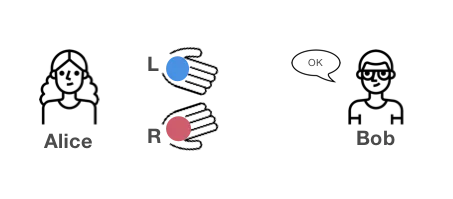
\includegraphics[width=0.5\textwidth]{images/balls1.png}
    \begin{columns}
        \begin{column}{0.45\textwidth}
            \centering
            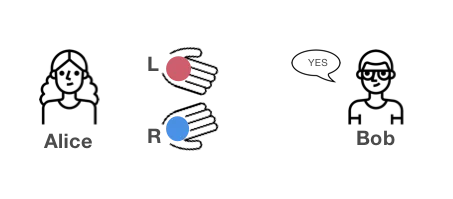
\includegraphics[height=0.45\textwidth]{images/balls2.png}            
        \end{column}
        \begin{column}{0.45\textwidth}
            \centering
            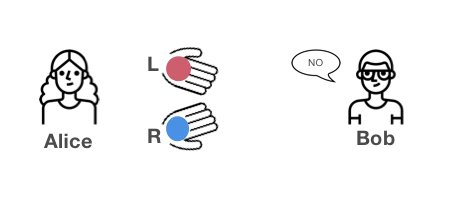
\includegraphics[height=0.45\textwidth]{images/balls3.png}            
        \end{column}
    \end{columns}
    \blfootnote{\cite{Ball} Understanding Zero-Knowledge Proofs through Simple Examples.}
\end{frame}

% ####################

\begin{frame}[fragile]{Motivación}
    \begin{columns}
        \begin{column}{0.45\textwidth}
            \begin{figure}
                \centering
                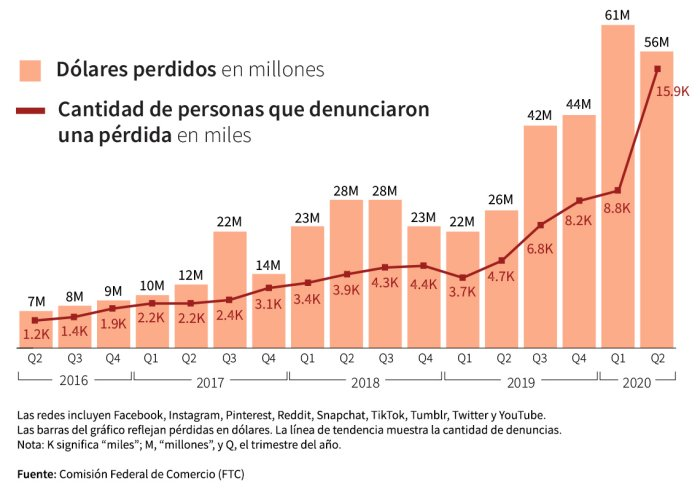
\includegraphics[width=0.9\textwidth]{images/scams.jpg}
                \caption{Fraudes \cite{Fraudes}} 
            \end{figure}
        \end{column}
        \begin{column}{0.45\textwidth}
            \centering
            \begin{figure}
                \centering
                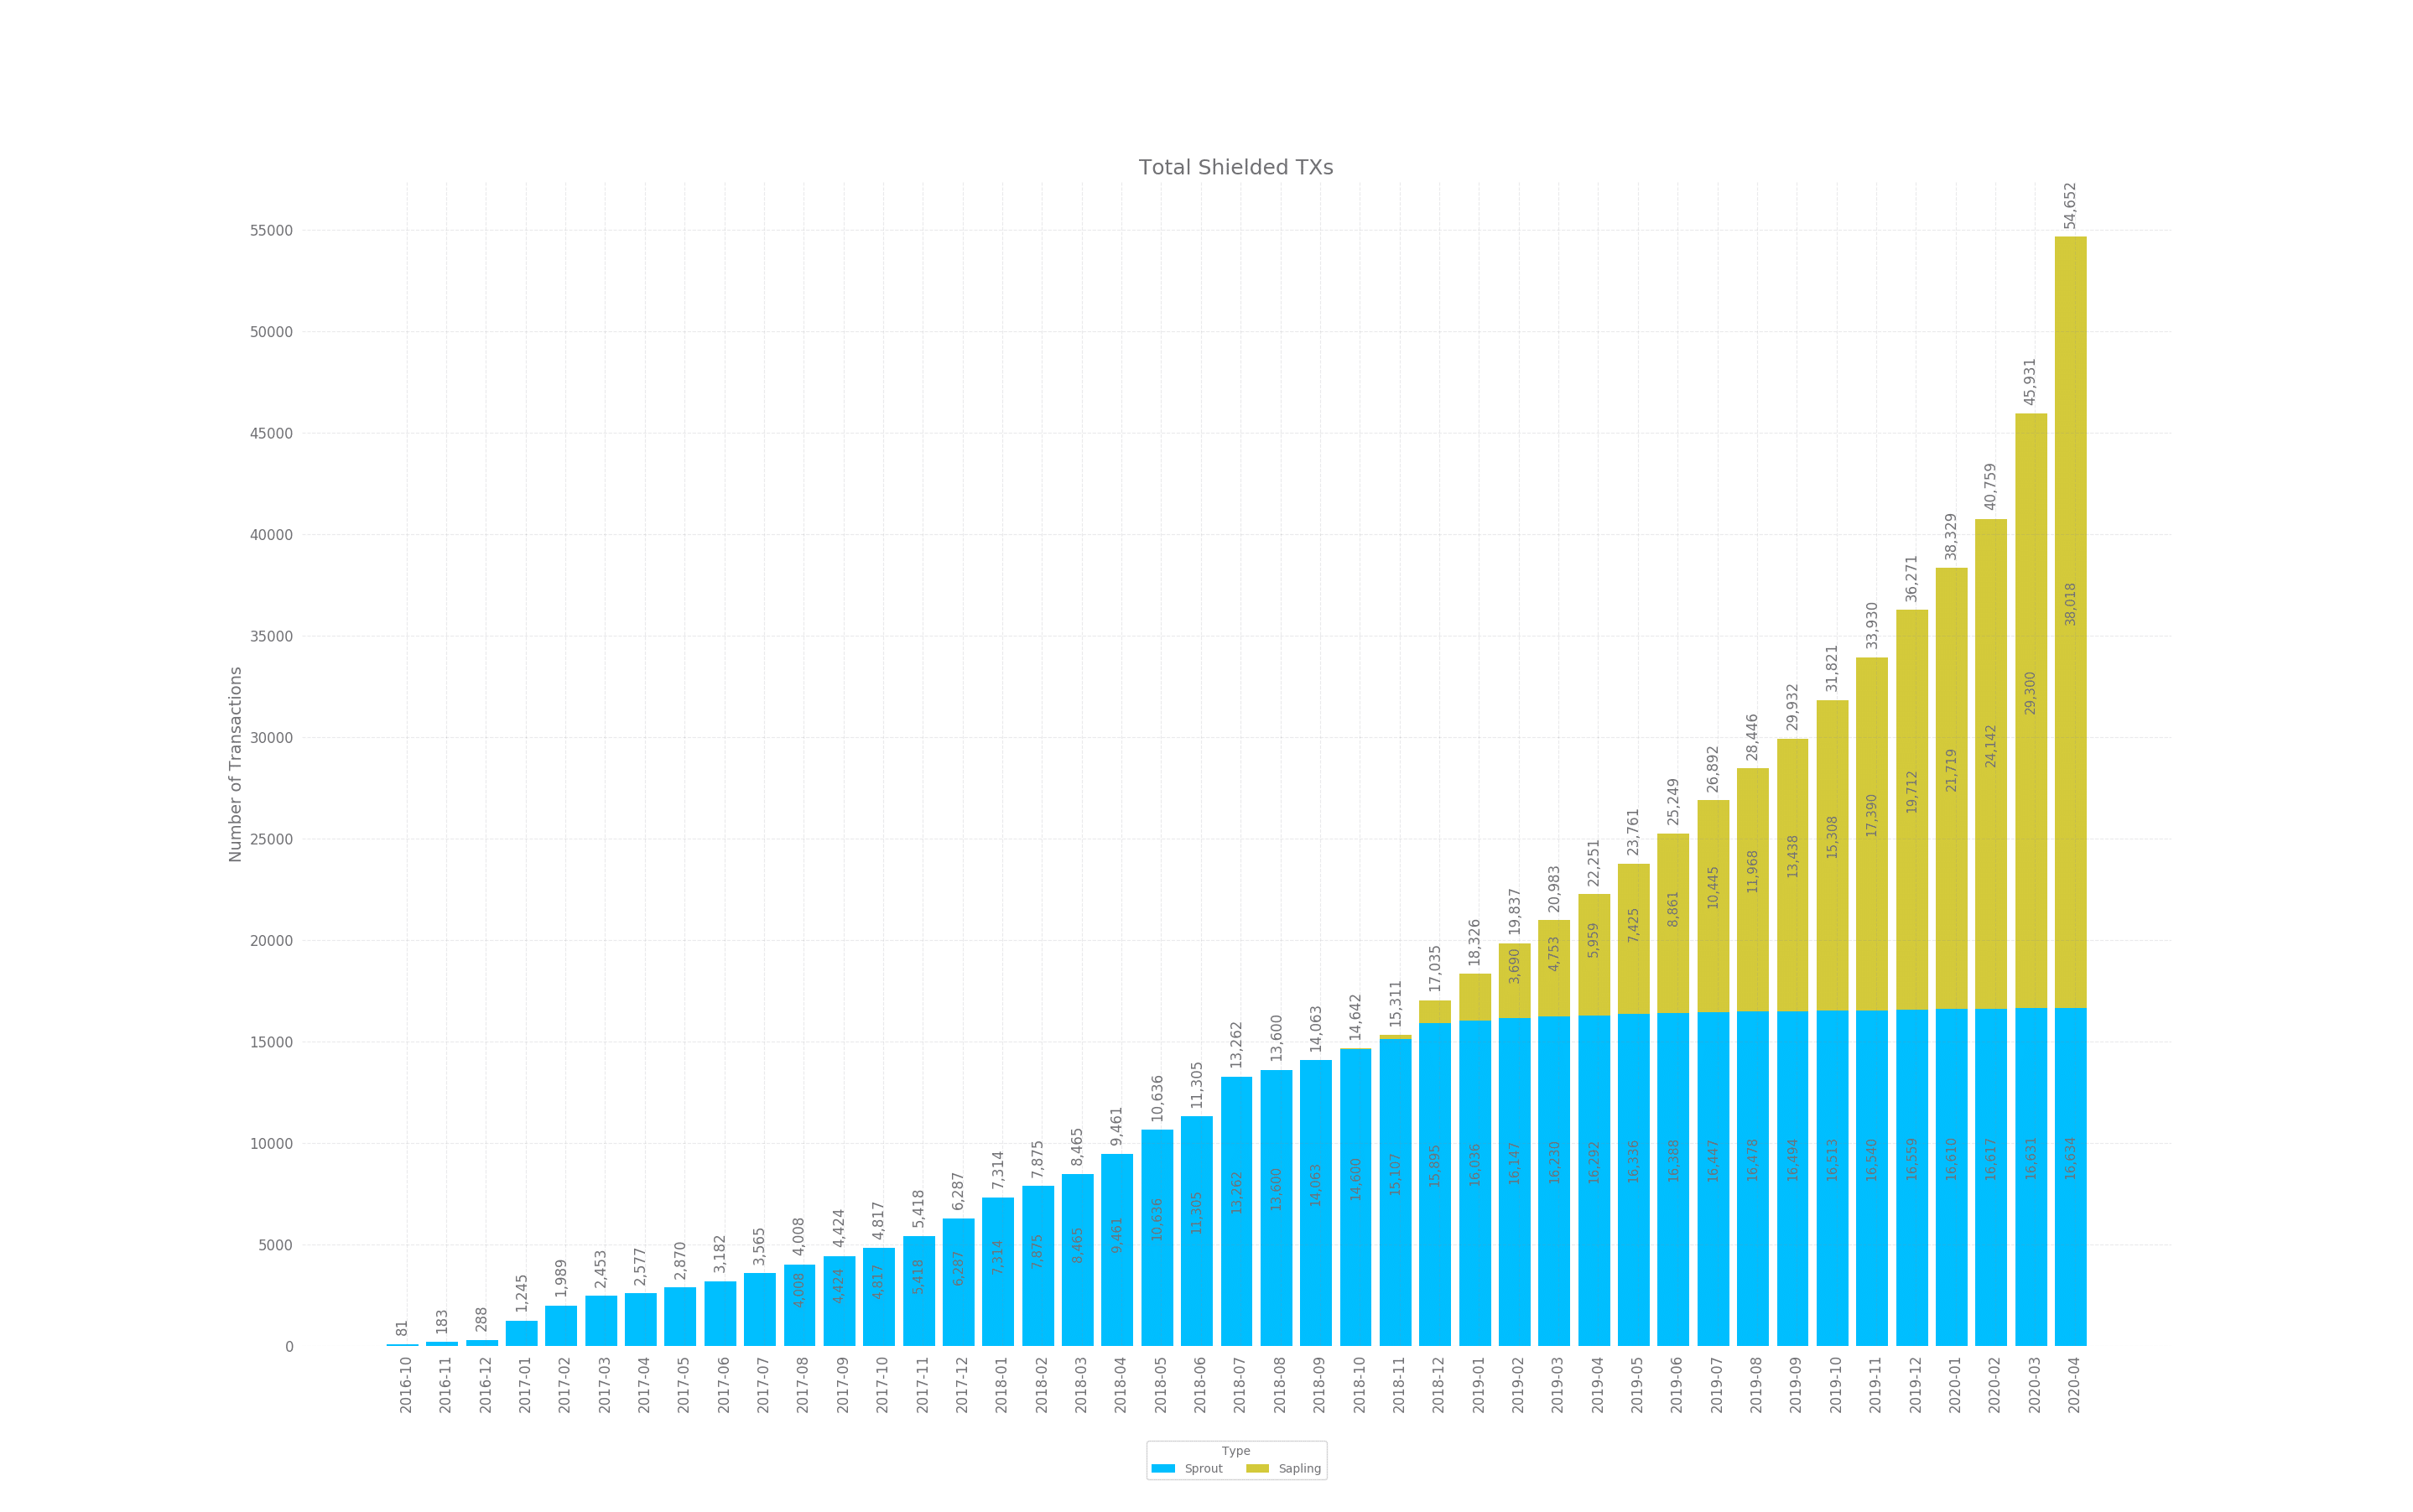
\includegraphics[width=0.85\textwidth]{images/zcash.png}  
                \caption{Zcash \cite{zCash}}
            \end{figure}
            \begin{figure}
                \centering
                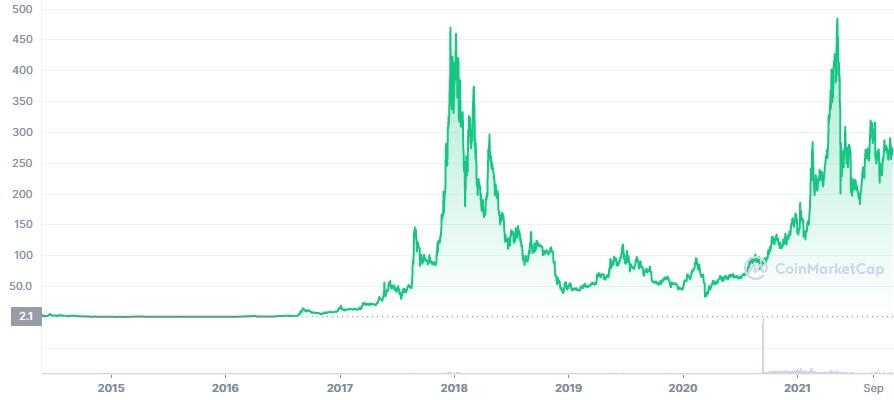
\includegraphics[width=0.85\textwidth]{images/monero.jpg}
                \caption{Monero \cite{Monero}} 
            \end{figure}     
        \end{column}
    \end{columns}
    \blfootnote{\cite{Fraudes} Se Disparan Los Fraudes En Instragram Por La Pandemia.}
    \blfootnote{\cite{zCash} Zcash Privacy Remains Strongest of Any Cryptocurrency, Even with Recent Chainalysis, Elliptic Support}
    \blfootnote{\cite{Monero} Monero (XMR) Price Prediction for 2023, 2024-2025 and Beyond}
\end{frame}

% ####################

\begin{frame}[fragile]{Aplicaciones}
    \begin{itemize}
        \item Pagos anónimos.
        \item Autenticación.
        \item Más de 18 ZKRP.
        \item Know Your Customer (KYC).
        \item Evaluación del riesgo hipotecario.
        \item Calificación y grado de inversión.
        \item Voto electrónico.
        \item Subastas y adquisiciones electrónicas.
    \end{itemize}
\end{frame}

% ####################

\begin{frame}[fragile]{Objetivos}
    Implementación de una herramienta que facilite el estudio de las pruebas de conocimiento cero.
    
    Para ello, queremos:
    \begin{itemize}
        \item Conocer el funcionamiento y algunas de las posibles aplicaciones de los protocolos de conocimiento cero.
        \item Desarrollar una herramienta que permita al usuario experimentar con los protocolos de conocimiento cero.
        \item Verificar el funcionamiento correcto se espera de dichos algoritmos.
    \end{itemize}
\end{frame}

% ####################

\section{Teoría}

\begin{frame}[fragile]{Marco histórico}
    Concebidas por primera vez en 1985 por Shafi Goldwasser, Silvio Micali y Charles Rackoff en el artículo \textit{The Knowledge Complexity of Interactive Proof-Systems} \cite{Historia}.

    \begin{center}
        \textit{De particular interés es el caso donde [...] mostramos que es posible probar interactivamente que un número es cuadrático sin residuo mod m liberando 0 conocimiento adicional.}
    \end{center}

    \vspace{0.25cm}
    
    \begin{columns}
        \begin{column}{0.7\textwidth}
            Oded Goldreich, Silvio Micali y Avi Wigderson demostraron que se puede crear un sistema de prueba de conocimiento cero para el problema de coloreado de gráficos NP completos con tres colores.
        \end{column}
        \begin{column}{0.25\textwidth}
            \begin{figure}
                \centering
                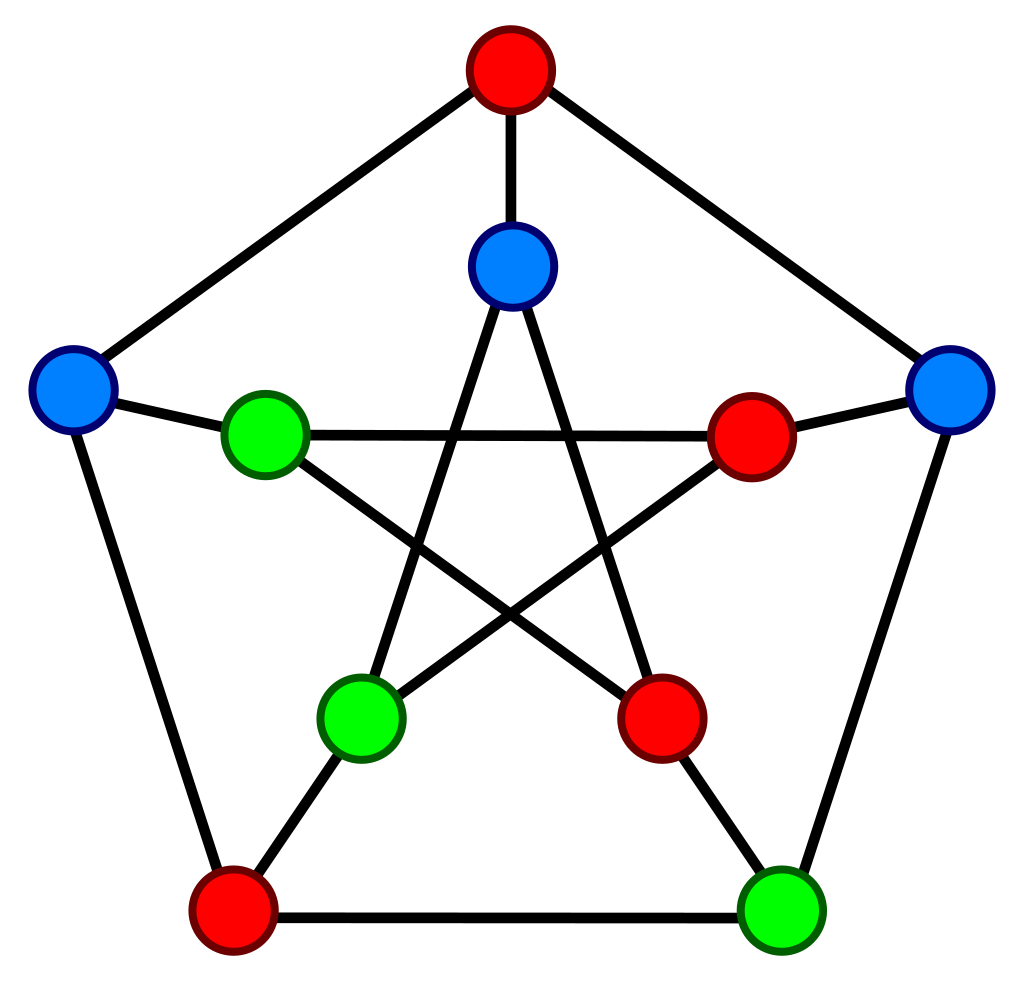
\includegraphics[width=0.85\textwidth]{images/grafos.png}
            \end{figure}
        \end{column}
    \end{columns}

    \vspace{0.25cm}
    
    \begin{columns}
        \begin{column}{0.6\textwidth}
            También demostraron que el problema de no isomorfismo de gráficos, el complemento del problema de isomorfismo de gráficos, tiene una prueba de conocimiento cero.
        \end{column}
        \begin{column}{0.35\textwidth}
            \begin{figure}
                \centering
                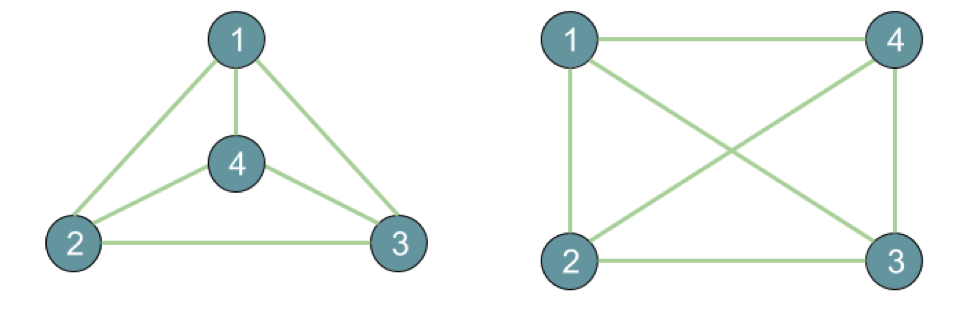
\includegraphics[width=0.95\textwidth]{images/isomorfismo.png}
            \end{figure}            
        \end{column}
    \end{columns}
\end{frame}

% ####################

\begin{frame}[fragile]{Protocolos de conocimiento cero en el contexto docente}
    Existencia de diversos artículos, pero todos centrados en su funcionamiento o en comparar diversos algoritmos:
    \begin{itemize}
        \item \textit{Efficient Proofs that a Committed Number Lies in an Interval} \cite{Boudot}
        \item \textit{A Survey on Zero Knowledge Range Proofs and Applications} \cite{Survey}
        \item \textit{Sharp: Proceedings of the 2022 ACM SIGSAC Conference on Computer and Communications Security} \cite{Sharp}
        \item \textit{Bulletproofs: Short proofs for confidential transactions and more} \cite{Bulletproofs}
    \end{itemize}
\end{frame}

% ####################

\begin{frame}[fragile]{Definición}
    Una prueba de conocimiento cero permite probar la verdad de una declaración sin compartir el contenido de la declaración o revelar cómo descubrió la verdad.
    \begin{itemize}
        \item \textbf{Completitud:} Si la entrada es válida, el protocolo de conocimiento cero siempre devuelve ``verdadero''.
        \item \textbf{Solidez:} Si la entrada no es válida, es teóricamente imposible engañar al protocolo de conocimiento cero para que devuelva ``verdadero''.
        \item \textbf{Conocimiento cero:} El verificador no aprende nada sobre una declaración más allá de su validez o falsedad.
    \end{itemize}
\end{frame}

% ####################

\begin{frame}[fragile]{Definición}
    Dado $x \in \mathcal{L}$, el probador es capaz de convencer a un verificador de que $x$ pertenece a $\mathcal{L}$, es decir, existe un testigo $w$ para $x$.
    \begin{itemize}
        \item \textbf{Setup:} Generación de parámetros: $params = \operatorname{Setup(\lambda)}$.
        \item \textbf{Prove:} Genera la prueba de conocimiento cero: $proof = \operatorname{Prove}(x, w)$
        \item \textbf{Verify:} Acepta o rechaza la prueba $proof$.
    \end{itemize}

    Con estos términos, una prueba de conocimiento cero cumple:
    \begin{itemize}
        \item \textbf{Completitud:} 
        $$Verify(Prove(x, w)) = 1$$
        \item \textbf{Solidez:}
        $$P[Verify(Prove(x, w)) = 1] \text{ es suficientemente baja.}$$
        \item \textbf{Conocimiento cero:} El verificador no aprende nada sobre una declaración más allá de su validez o falsedad.
    \end{itemize}
\end{frame}

% ####################

\begin{frame}[fragile]{Pruebas interactivas y no interactivas}
    \begin{columns}
        \begin{column}{0.45\textwidth}
            \centering
            \textbf{Pruebas interactivas}
            
            \vspace{0.25cm}
            
            \begin{figure}
                \centering
                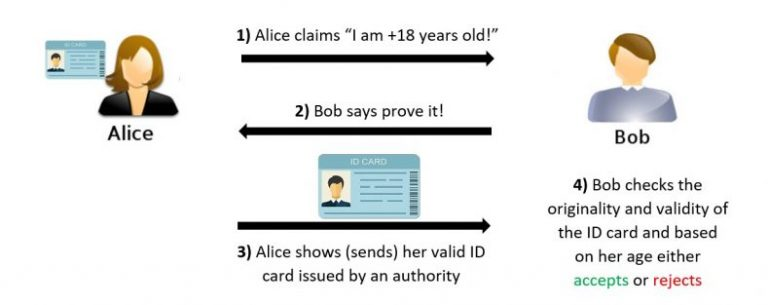
\includegraphics[width=0.95\textwidth]{images/zkp.jpg}
            \end{figure}
        \end{column}
        \begin{column}{0.45\textwidth}
            \textbf{Pruebas no interactivas}
            
            \vspace{0.25cm}
            
            Requieren sólo una ronda de comunicación entre los participantes (proveedor y verificador).
            
            \vspace{0.25cm}
            
            Una vez que se genera una prueba, está disponible para que cualquier otra persona (con acceso al algoritmo de verificación) la verifique.

        \end{column}
    \end{columns}
    
    \blfootnote{\cite{ZKP} CO6GC: Introduction to Zero-Knowledge Proofs (Part 1)}
\end{frame}

% ####################

\begin{frame}[fragile]{ZK-SNARK y ZK-STARK}
    ZK-SNARK (Zero-Knowledge Succinct Non-Interactive Argument of Knowledge):
    \begin{itemize}
        \item \textbf{Conocimiento cero:} Un verificador puede validar la integridad de una declaración sin saber nada más sobre la declaración.
        \item \textbf{Sucinto:} La prueba de conocimiento cero es más pequeña que el testigo y se puede verificar rápidamente.
        \item \textbf{No interactivo}: La prueba es no interactiva porque el probador y el verificador solo interactúan una vez.
        \item \textbf{Argumento:} La prueba satisface el requisito de solidez.
        \item \textbf{De conocimiento:} La prueba de conocimiento cero no puede construirse sin acceso a la información secreta.
    \end{itemize}

    ZK-STARK (Zero-Knowledge Scalable Transparent Argument of Knowledge):
    \begin{itemize}
        \item \textbf{Escalable:} Es más rápido que ZK-SNARK en la generación y verificación de pruebas cuando el tamaño del testigo es mayor.
        \item \textbf{Transparente:} Se basa en la aleatoriedad verificable públicamente para generar parámetros.
    \end{itemize}
\end{frame}

% ####################

\begin{frame}[fragile]{Zero Knowledge Range Proof}
    Permiten probar que un valor entero secreto pertenece a un intervalo.

    \begin{itemize}
        \item Propuestas de representación entera:
        \begin{itemize}
            \item \textbf{Descomposición cuadrada (\textit{Square decomposition}):} Para probar que $x \in [a, b]$ es equivalente probar que $x - a \geq 0$ y que $b - x \geq 0$.
            \item \textbf{Basado en firma (\textit{Signature-based})}.
        \end{itemize}
        \item Propuestas de representación binaria:
        \begin{itemize}
            \item \textbf{Decomposición multi-base (\textit{Multi-base decomposition}):} Utiliza aritmética booleana.
            \item \textbf{Compromisos homomórficos de dos niveles (\textit{Two-tiered homomorphic commitments}):} Utiza \textit{batches} de elementos de $\mathbb{Z}_{p}$.
            \item \textbf{\textit{Bulletproofs}:} El probador convence a un verificador de que conoce vectores cuyo producto interno es igual a un valor público determinado.
        \end{itemize}
    \end{itemize}

\end{frame}

% ####################

\begin{frame}[fragile]{Descomposición cuadrada (\textit{Square Decomposition})}
    Sea un entero positivo $x$, y sea $E = g^{x}h^{r} (\operatorname{mod} \text{ n})$, y supongamos que se quiere probar que $x \in [a, b]$.

    Se escribe el entero positivo $x - a$ como la suma del cuadrado mayor menor que $x$, $x_{1}^{2}$, y de $\rho$, un número positivo. Luego se selecciona aleatoriamente $r_{1}, r_{2} \in [0, 2^{s}n-1]$ de modo que $r_{1} + r_{2} = r$, y se calculan:
    $$E_{1} = g^{x_{1}^{2}}h^{r_{1}} (\operatorname{mod} \text{ n}) \hspace{1cm} \text{y} \hspace{1cm} E_{2} = g^{\rho}h^{r_{2}} (\operatorname{mod} \text{ n})$$

    Por lo tanto:
    $$E_{1}E_{2} = g^{x_{1}^{2}+\rho}h^{r_{1}+r_{2}} (\operatorname{mod} \text{ n}) = g^{x-a}h^{r} (\operatorname{mod} \text{ n}) \hspace{1cm} \text{y} \hspace{1cm} x - a \geq 0$$

    Demostrando que $E_{1}$ oculta un cuadrado y que $E_{2}$ oculta un número menor que $2^{t+\ell+1}\sqrt{b-a}$, y aplicando el mismo método para $b - x$, se prueba que:
    $$x \in [a - 2^{t+\ell+1} \sqrt{b-a}, b + 2^{t+\ell+1} \sqrt{b-a}]$$
\end{frame}

% ####################

\begin{frame}[fragile]{Teorema extendido de Euclides}
    $$mcd(a, b) = r_{n}$$
    \begin{table}[ht]
        \centering
        \begin{tabular}{c c|c c}
             & a & 1 & 0 \\
             & b & 0 & 1 \\
             $q_{2}$ & $r_{3}$ & $u_{3} = 1 - 0 \cdot q_{2}$ & $v_{3} = 0 - q_{2} \cdot 1$ \\
             $\dots$ & $\dots$ & $\dots$ & $\dots$ \\
             $q_{i-2}$ & $r_{i-1}$ & $u_{i-1}$ & $v_{i-1}$ \\
             $q_{i-1}$ & $r_{i}$ & $u_{i}$ & $v_{i}$ \\
             $q_{i}$ & $r_{i+1}$ & $u_{i+1} = u_{i-1} - u_{i} \cdot q_{i}$ & $v_{i+1} = v_{i-1} - q_{i} \cdot v_{i}$ \\
             $\dots$ & $\dots$ & $\dots$ & $\dots$ \\
        \end{tabular}
        \caption{Algoritmo extendido de Euclides}
    \end{table}
    $$1 = mcd(a, n) = u \cdot a + v \cdot n \equiv u \cdot a (\operatorname{mod} \text{ n})$$
\end{frame}

% ####################

\begin{frame}[fragile]{Pruebas y verificaciones}
    \begin{columns}
        \begin{column}{0.45\textwidth}
            \begin{figure}
                \centering
                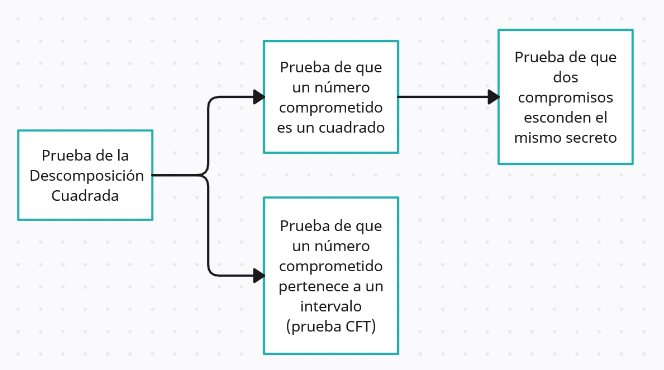
\includegraphics[width=0.95\textwidth]{images/Esquema Prueba.png}
                \caption{Esquema de pruebas}
            \end{figure}
        \end{column}
        \begin{column}{0.45\textwidth}
            \begin{figure}
                \centering
                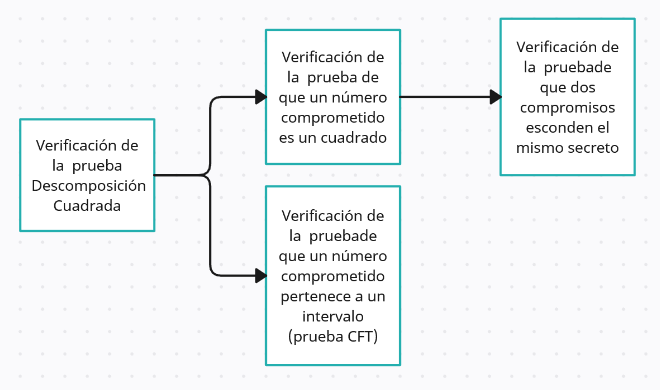
\includegraphics[width=0.95\textwidth]{images/Esquema Verificacion.png}
                \caption{Esquema de verificaciones}
            \end{figure}
        \end{column}
    \end{columns}
\end{frame}

% ####################

\begin{frame}[fragile]{Selección de algoritmo}
    \begin{columns}
        \begin{column}{0.45\textwidth}
            \begin{figure}
                \centering
                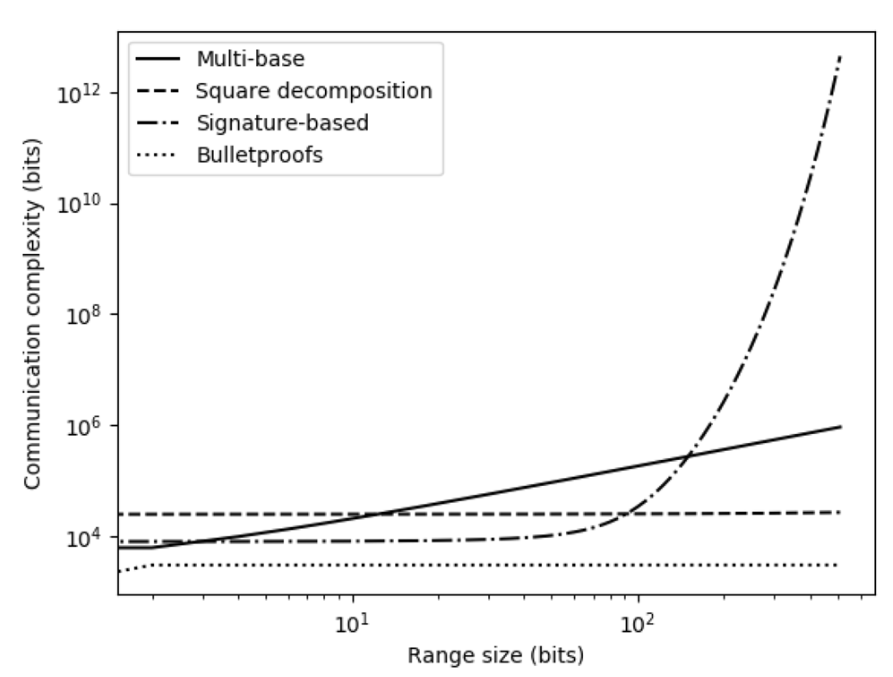
\includegraphics[width=0.95\textwidth]{images/proofsSize.png}
            \end{figure}
        \end{column}
        \begin{column}{0.45\textwidth}
            \begin{figure}
                \centering
                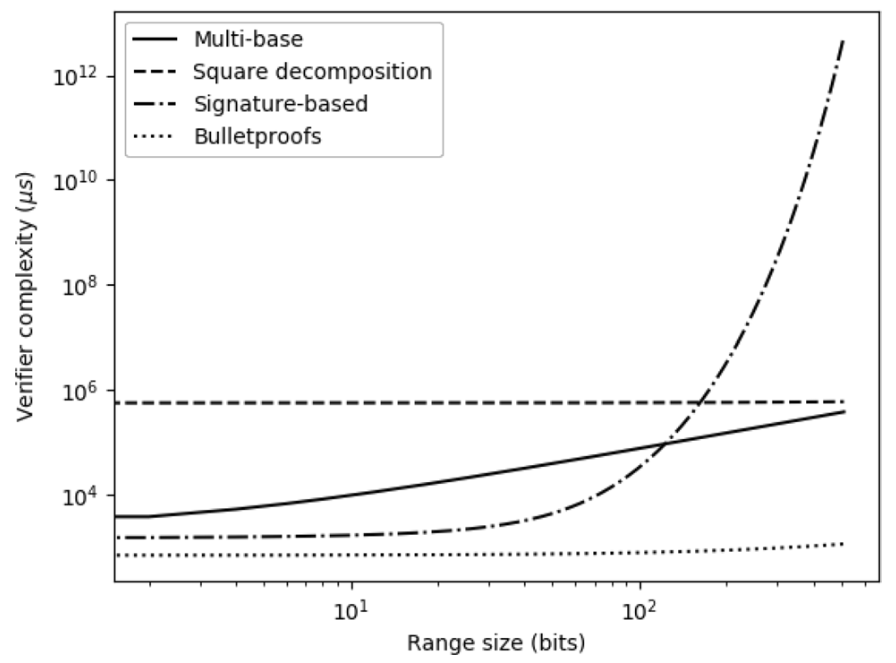
\includegraphics[width=0.95\textwidth]{images/verifierComplexity.png}
            \end{figure}
            \begin{figure}
                \centering
                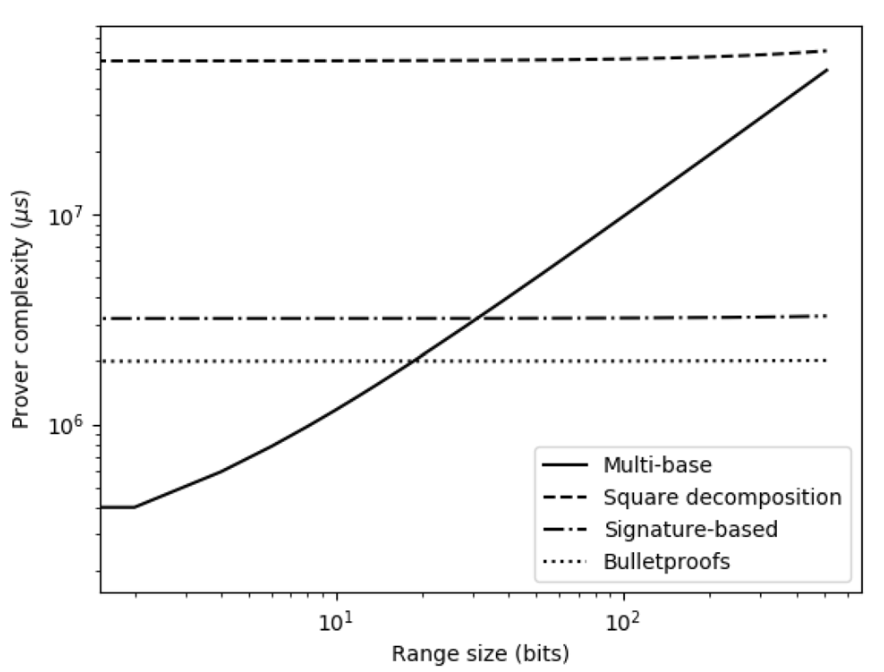
\includegraphics[width=0.95\textwidth]{images/proverComplexity.png}
            \end{figure}
        \end{column}
    \end{columns}
    
    \blfootnote{\cite{Survey} A Survey on Zero Knowledge Range Proofs and Applications - SN Applied Sciences.}
\end{frame}

% ####################

\begin{frame}[fragile]{Bulletproofs vs Sharp}
    \begin{figure}
        \centering
        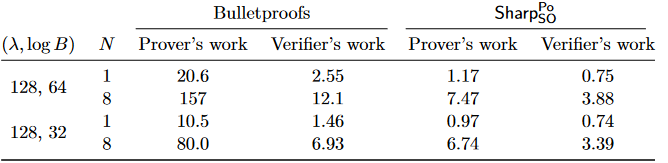
\includegraphics[width=0.95\textwidth]{images/sharp vs bulletproof.png}
    \end{figure}
    
    \blfootnote{\cite{Sharp} Sharp: Proceedings of the 2022 ACM SIGSAC Conference on Computer and Communications Security.}
\end{frame}

% ####################


\section{Implementación}

\begin{frame}[fragile]{Implementación}
    \begin{columns}
        \begin{column}{0.45\textwidth}
            \begin{figure}
                \centering
                
\includegraphics[width=0.5\textwidth]{images/python.png}
            \end{figure}
            \vspace{1.5cm}
            \begin{figure}
                \centering
                
\includegraphics[width=0.8\textwidth]{images/flask.png}
            \end{figure}
        \end{column}
        \begin{column}{0.45\textwidth}
            \begin{figure}
                \centering
                
\includegraphics[width=0.5\textwidth]{images/html-5.png}
            \end{figure}
            \vspace{1.5cm}
            \begin{figure}
                \centering
                
\includegraphics[width=0.8\textwidth]{images/bulma-banner.png}
            \end{figure}
        \end{column}
    \end{columns}
\end{frame}

% ####################

\begin{frame}[fragile]{Esquema de la interfaz web}
    \begin{figure}
        \centering
        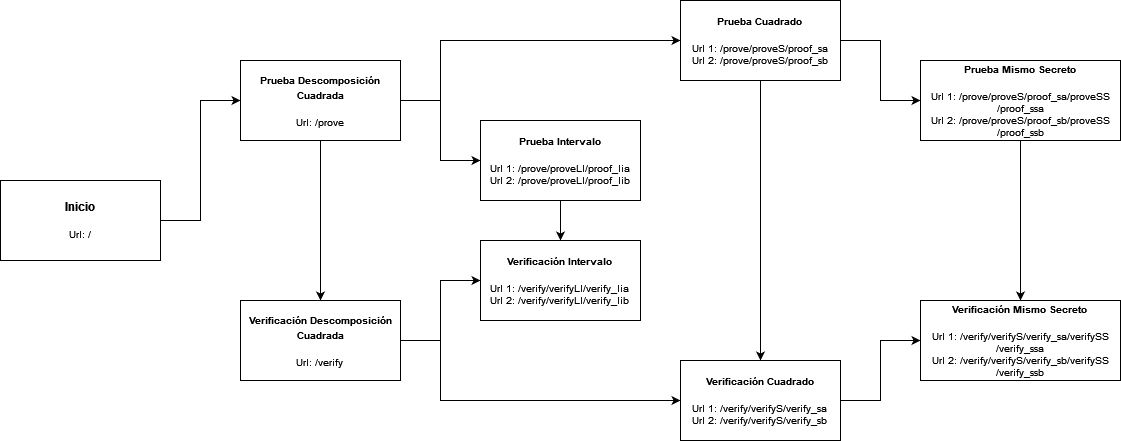
\includegraphics[width=\textwidth]{images/Esquema.png}
    \end{figure}
\end{frame}

% ####################

\begin{frame}[fragile]{Interfaz web}
    \begin{figure}
        \centering
        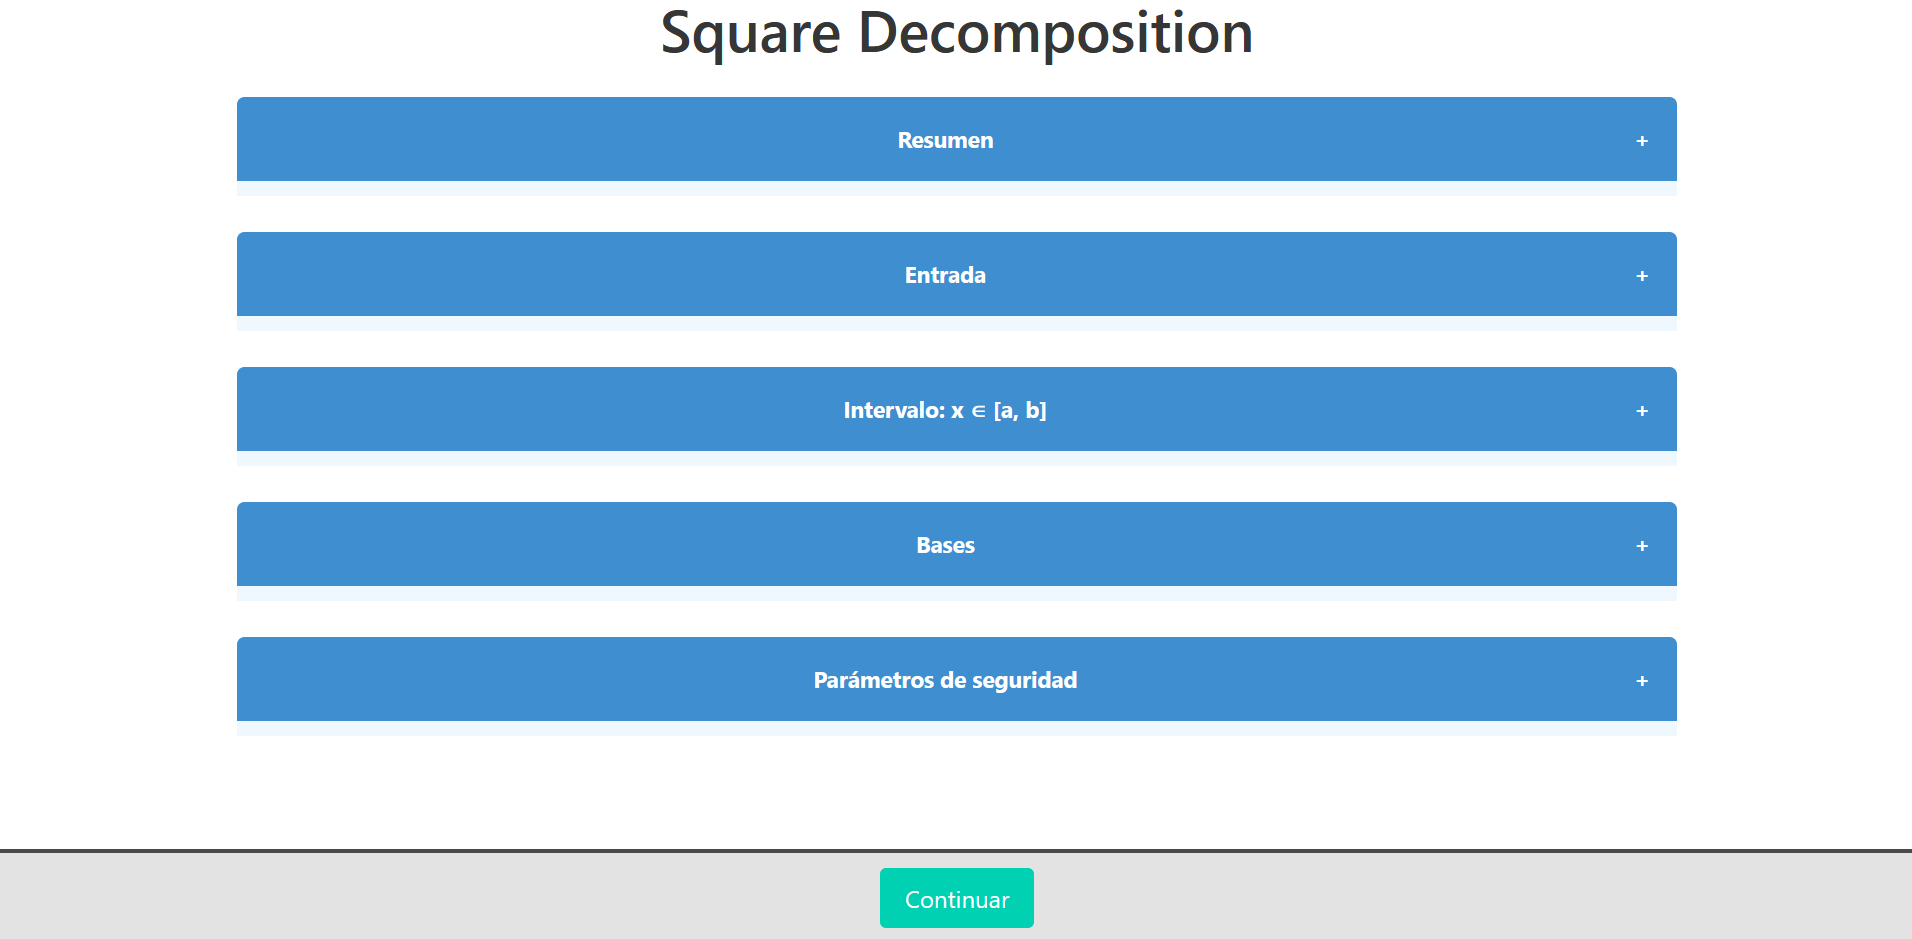
\includegraphics[width=\textwidth]{images/input.png}
    \end{figure}
\end{frame}

% ####################

\begin{frame}[fragile]{Pruebas funcionales}
    \begin{columns}
        \begin{column}{0.45\textwidth}
            \begin{figure}
                \centering
                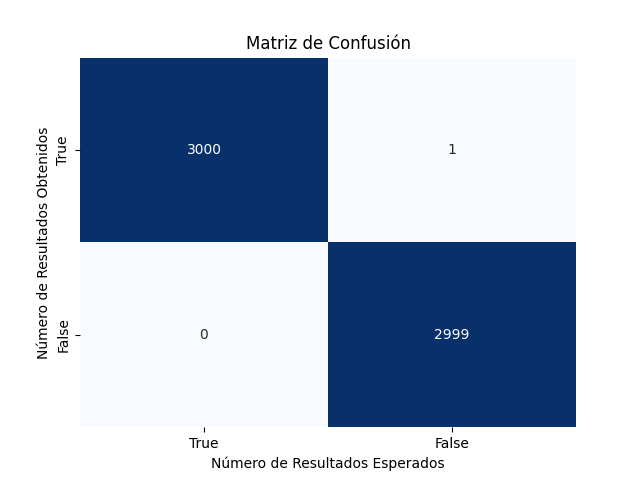
\includegraphics[width=\textwidth]{images/Resultados test.png}
                \caption{Resultados de una ejecución}
            \end{figure}
        \end{column}
        \begin{column}{0.45\textwidth}
            \begin{figure}
                \centering
                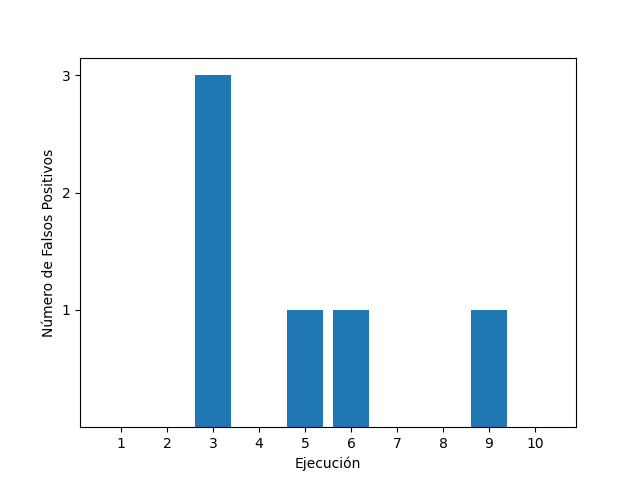
\includegraphics[width=\textwidth]{images/resultados.png}
                \caption{Resultados de 10 ejecuciones}
            \end{figure}
        \end{column}
    \end{columns}
\end{frame}

% ####################

\begin{frame}[fragile]{Tiempo de verificación}
    \begin{figure}
        \centering
        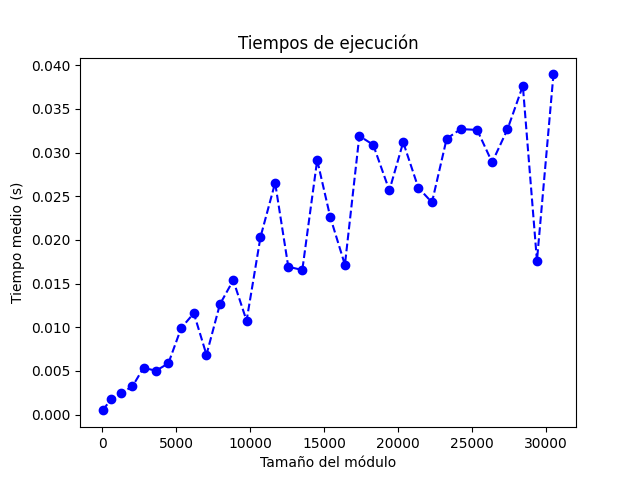
\includegraphics[width=\textwidth]{images/tiempos.png}
    \end{figure}
\end{frame}

% ####################

\begin{frame}[fragile]{Regresión}
    \begin{figure}
        \centering
        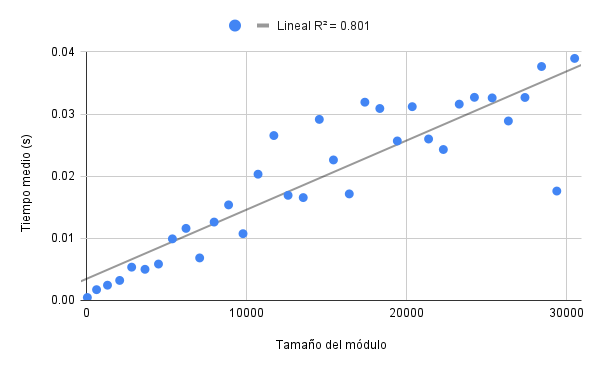
\includegraphics[width=0.45\textwidth]{images/lineal.png}
    \end{figure}
    \begin{columns}
        \begin{column}{0.45\textwidth}
            \begin{figure}
                \centering
                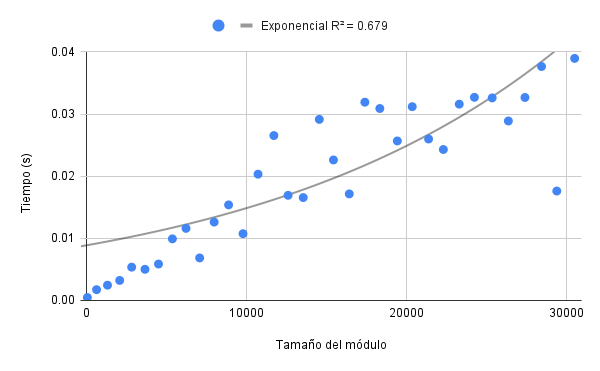
\includegraphics[width=\textwidth]{images/exponencial}
            \end{figure}
        \end{column}
        \begin{column}{0.45\textwidth}
            \begin{figure}
                \centering
                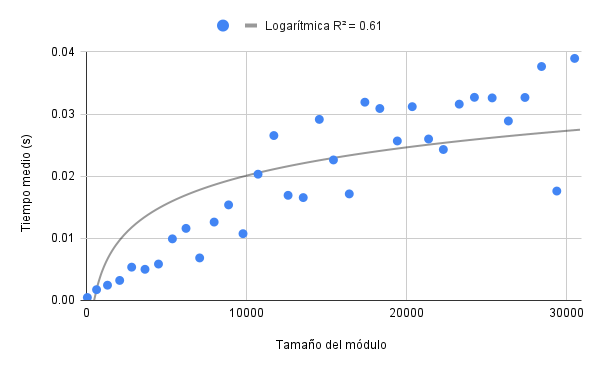
\includegraphics[width=\textwidth]{images/logaritmica.png}
            \end{figure}
        \end{column}
    \end{columns}
\end{frame}

% ####################

\section{Conclusiones y Líneas de Trabajo Futuro}

\begin{frame}[fragile]{Conclusiones}
    Con este trabajo se han logrado los siguientes objetivos:
    \begin{itemize}
        \item Estudio de los protocolos de conocimiento cero.
        \item Comparación entre los distintos algoritmos.
        \item Estudio en detalle del algoritmo de la Descomposición Cuadrada.
        \item Implementación del algoritmo.
        \item Desarrollo de una herramienta docente.
        \item Pruebas funcionales.
    \end{itemize}
\end{frame}

% ####################

\begin{frame}[fragile]{Líneas de Trabajo Futuro}
    \begin{itemize}
        \item Estudiar otros algoritmos ZKP.
    
        \item Solucionar las pruebas falsas clasificadas como verdaderas.
        \begin{itemize}
            \item Errores debidos a la tolerancia.
            \item Errores debidos a la aleatoriedad.
        \end{itemize}
    \end{itemize}
\end{frame}

% ####################

\appendix
\backupbegin

\begin{frame}[allowframebreaks]{Referencias}
    \setbeamertemplate{bibliography item}[text]
    \import{./Latex/}{referencias.tex}
\end{frame}

\backupend
\end{document}